Den strategi som vann flest poäng var tit-for-tat, som samlade ihop drygt 30000 poäng. Figur \ref{points} nedan beskriver hur många poäng varje strategi samlade ihop. 
\begin{figure}[htb]
	\begin{center}
	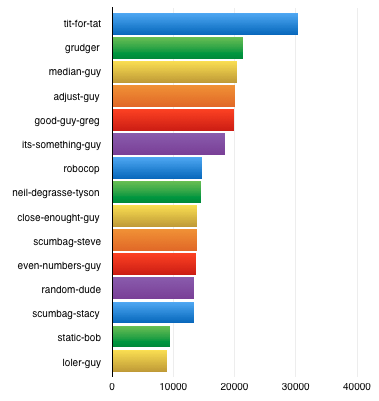
\includegraphics[scale=0.75, angle=0]{bilder/points.png}
	\caption{Totalt antal poäng efter 1000 omgångar.}
	\label{points}
	\end{center}
\end{figure}

Den strategi som vann flest gånger var också tit-for-tat. Figur 2 nedan beskriver hur många vinster respektive strategi tog. Topp tre i figur \ref{points} och figur \ref{wins} består av samma strategier. Strategierna tit-for-tat, grudger och Median guy är med andra ord både pålitliga och effektiva. 
\begin{figure}[htb]
	\begin{center}
	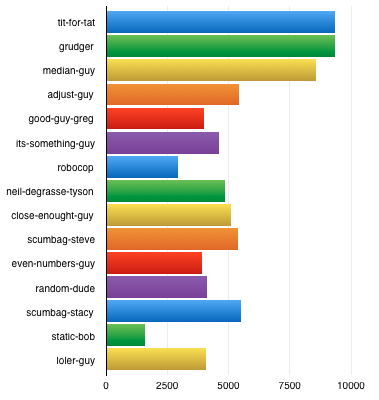
\includegraphics[scale=0.75, angle=0]{bilder/wins.png}
	\caption{Totalt antal vinster efter 1000 omgångar.}
	\label{wins}
	\end{center}
\end{figure}

Gemensamt för de tre bästa strategierna är att de tar hänsyn till motståndarens historik. Gemensamt är också att tit-for-tat och grudger startar alltid på 10 och median-guy startar på ett slumpmässigt tal, vilket kan vara 10. 

\begin{figure}[htb]
	\begin{center}
	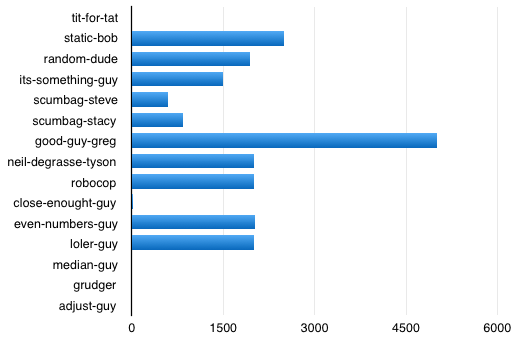
\includegraphics[scale=0.75, angle=0]{bilder/adjust-guy.png}
	\caption{Detta är bildtexten}
	\label{adjust-guy}
	\end{center}
\end{figure}

\begin{figure}[htb]
	\begin{center}
	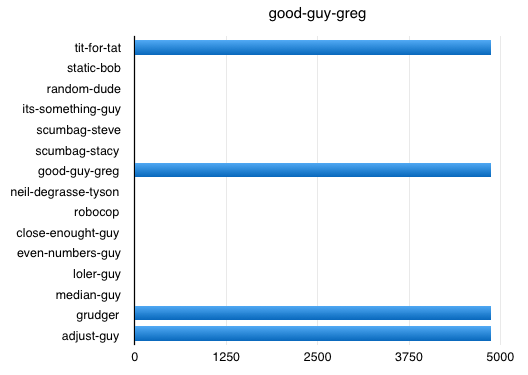
\includegraphics[scale=0.75, angle=0]{bilder/good-guy-greg.png}
	\caption{Detta är bildtexten}
	\label{good-guy-greg}
	\end{center}
\end{figure}

\begin{figure}[htb]
	\begin{center}
	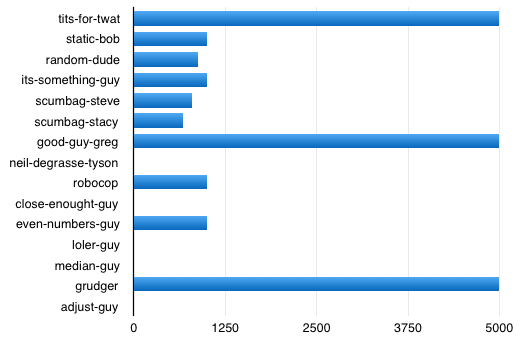
\includegraphics[scale=0.75, angle=0]{bilder/grudger.png}
	\caption{Detta är bildtexten}
	\label{grudger}
	\end{center}
\end{figure}

\begin{figure}[htb]
	\begin{center}
	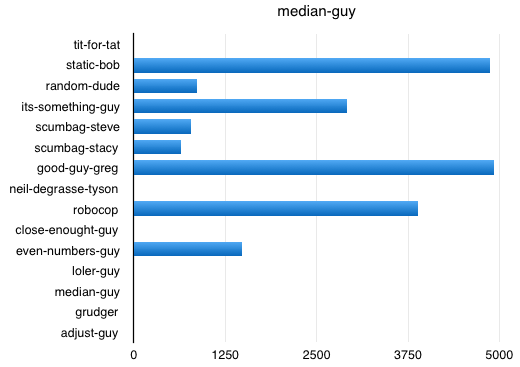
\includegraphics[scale=0.75, angle=0]{bilder/median-guy.png}
	\caption{Detta är bildtexten}
	\label{median-guy}
	\end{center}
\end{figure}

\begin{figure}[htb]
	\begin{center}
	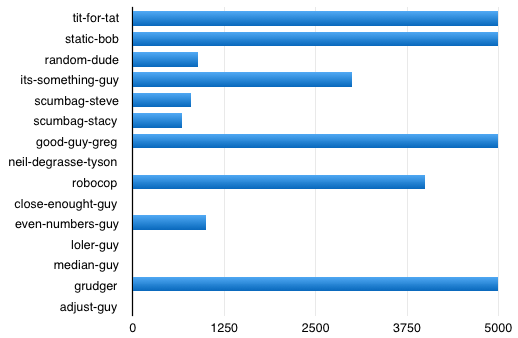
\includegraphics[scale=0.75, angle=0]{bilder/tit-for-tat.png}
	\caption{Detta är bildtexten}
	\label{tit-for-tat}
	\end{center}
\end{figure}